\section{Kinetically distinct phases of tau on microtubules regulate kinesin motors and severing enzymes}
\label{sec:tau}
\subsection{Tau has one diffusive and one cooperative microtubule binding mode}
\captionsetup[<float-type>]{list=no}
\begin{figure}[b!]
\centering
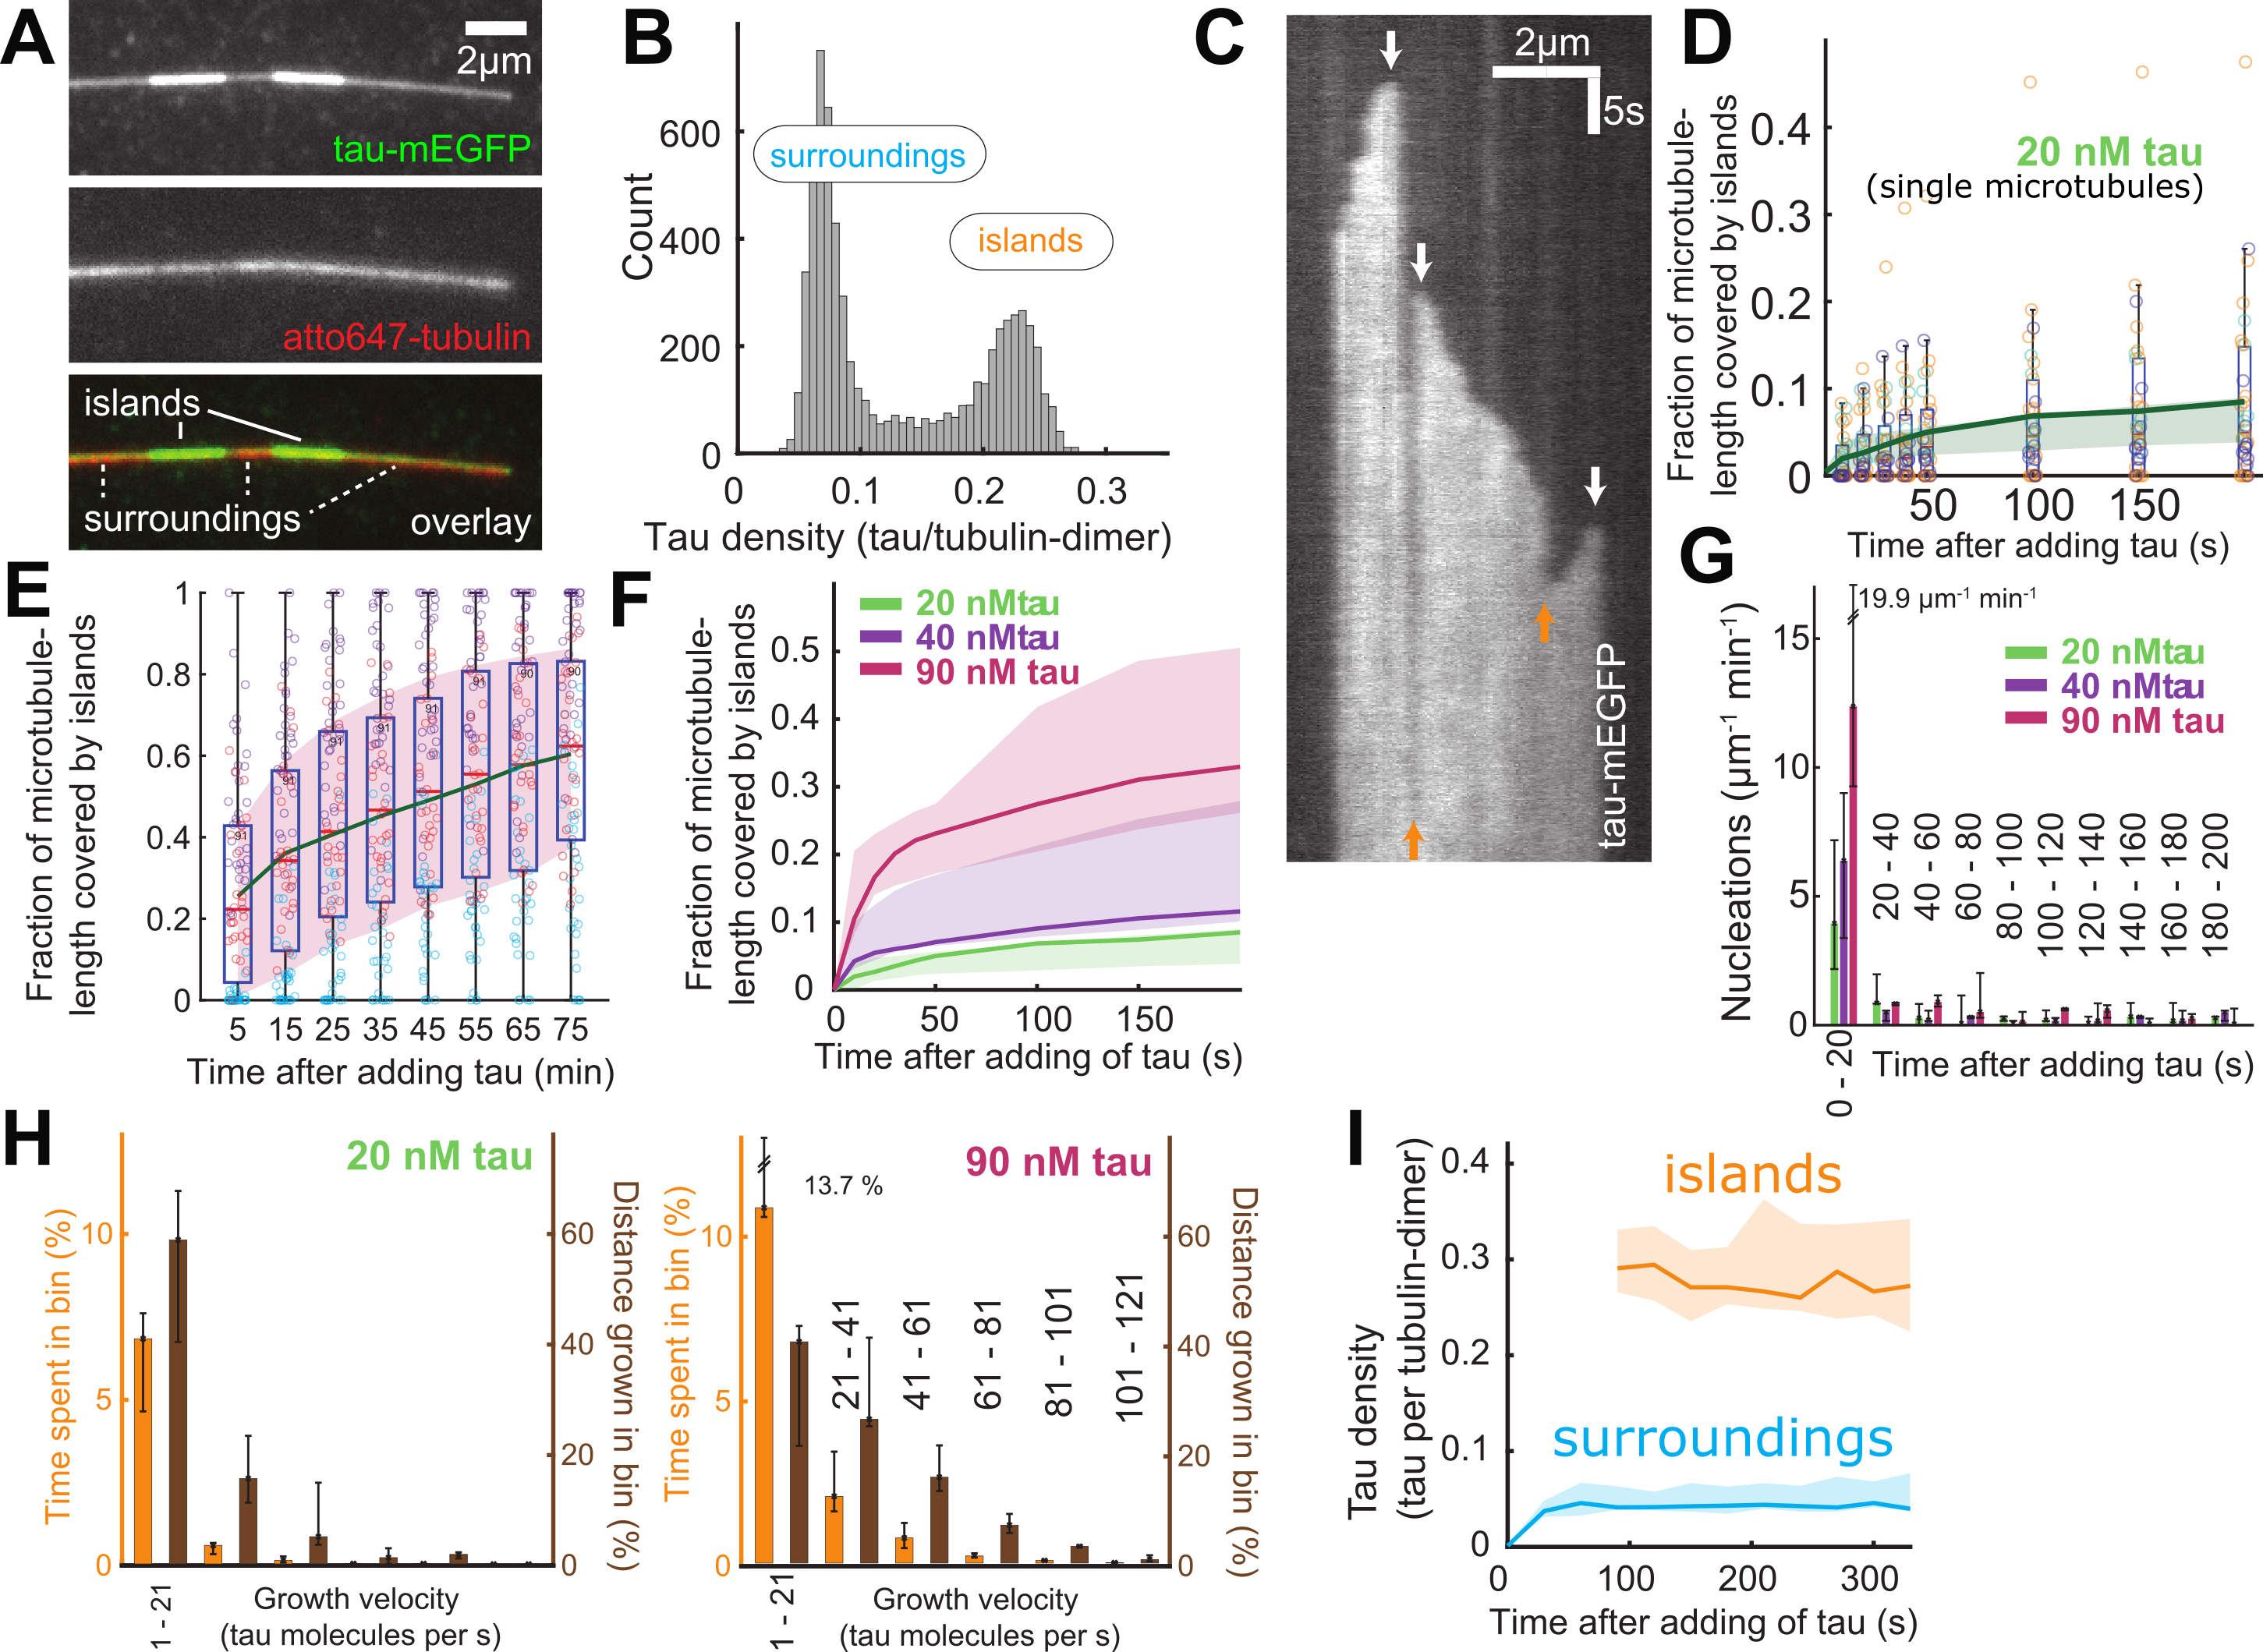
\includegraphics[width=1\linewidth]{Figures/tauGROW.png}
\end{figure}
\captionsetup[<float-type>]{list=yes}
\begin{figure}[t!]
\caption[Tau assembles into tau islands on microtubules.]{\textbf{Tau assembles into tau islands on microtubules.} (A) Multichannel fluorescence micrograph showing islands of high-density tau (bright green) surrounded by regions of low-density tau (dim green) on an Atto-647-labeled microtubule (red). Images taken 5 minutes after the addition of 20 nM tau. (B) Distribution of fluorescence intensity of tau along the microtubules such as shown in (A) showing two distinct populations. (C) Kymograph showing the fluorescence signal of tau on a microtubule after the addition 20 nM tau. Initially the microtubule is covered by low tau density. Over time, high-density tau islands start to assemble. White arrows indicate the nucleation points. Orange arrows indicate the merging of two neighboring islands growing towards each other. (D) Fraction of microtubule length covered by tau islands at different concentrations after the addition of tau at the time = 0. Boxplots represent the coverage statistics of individual microtubules. (E) Fraction of microtubule length covered by tau islands over time under different tau concentrations. Analogous to D, however, here coverage is computed over all microtubules in a given field of view (n = 3 experiments per condition, shaded area is drawn between experiment with least coverage and experiment with most coverage, line shows coverage in remaining experiment). (F) Distribution of time between the addition of tau and the formation of the islands (3 experiments per condition, n = 610 nucleation events). Bars show the median; error bars show the minimum and the maximum value. (G) Island assembly does not cease even 75 minutes after the addition of 20 nM tau. The same data representation as in D. (H) Histograms of island growth velocities at different tau concentrations in solution (Methods, n = 2131 velocity traces). The fractions of all bins, together with the fraction of time where growth halted (not shown), add up to 100\%. (I) Exemplary time-trace of the tau density in the islands and their surroundings (Methods) after the addition of tau (n = 5 microtubules; thick lines and shaded areas indicate median and first and third quartiles, respectively). This experiment was performed with lower frame rate than in C to minimize photo-bleaching.
	}\label{tauGROW}
\end{figure}

To study microtubule-associated tau molecules, we immobilized Atto-647-labeled microtubules on a coverslip, added full-length, human 2N4R (tau441) tau fluorescently labeled on the C-terminus (tau-mEGFP or tau-mCherry) and performed time-lapse imaging using TIRF microscopy (Methods). After the addition of 20 nM tau we observed on the microtubules the formation of high-density tau islands, surrounded by regions with low tau density \pref{tauGROW}{A-C}. These islands, after nucleating from diffraction-limited spots, grew along along a given microtubule to cover more and more of its length \pref{tauGROW}{C,D}. After 75 minutes, most of the microtubule length in a given field of view was covered with islands, with islands still continuing to grow \pref{tauGROW}{E}. When repeating this experiment with higher tau concentrations of 40 and 90nM, microtubules were covered more quickly \pref{tauGROW}{F}, due to a higher nucleation rate of islands \pref{tauGROW}{G} as well as due to faster and more consistent growth at island boundaries \pref{tauGROW}{H}. 

\begin{wrapfigure}{l}{0.6\textwidth}
	\centering
	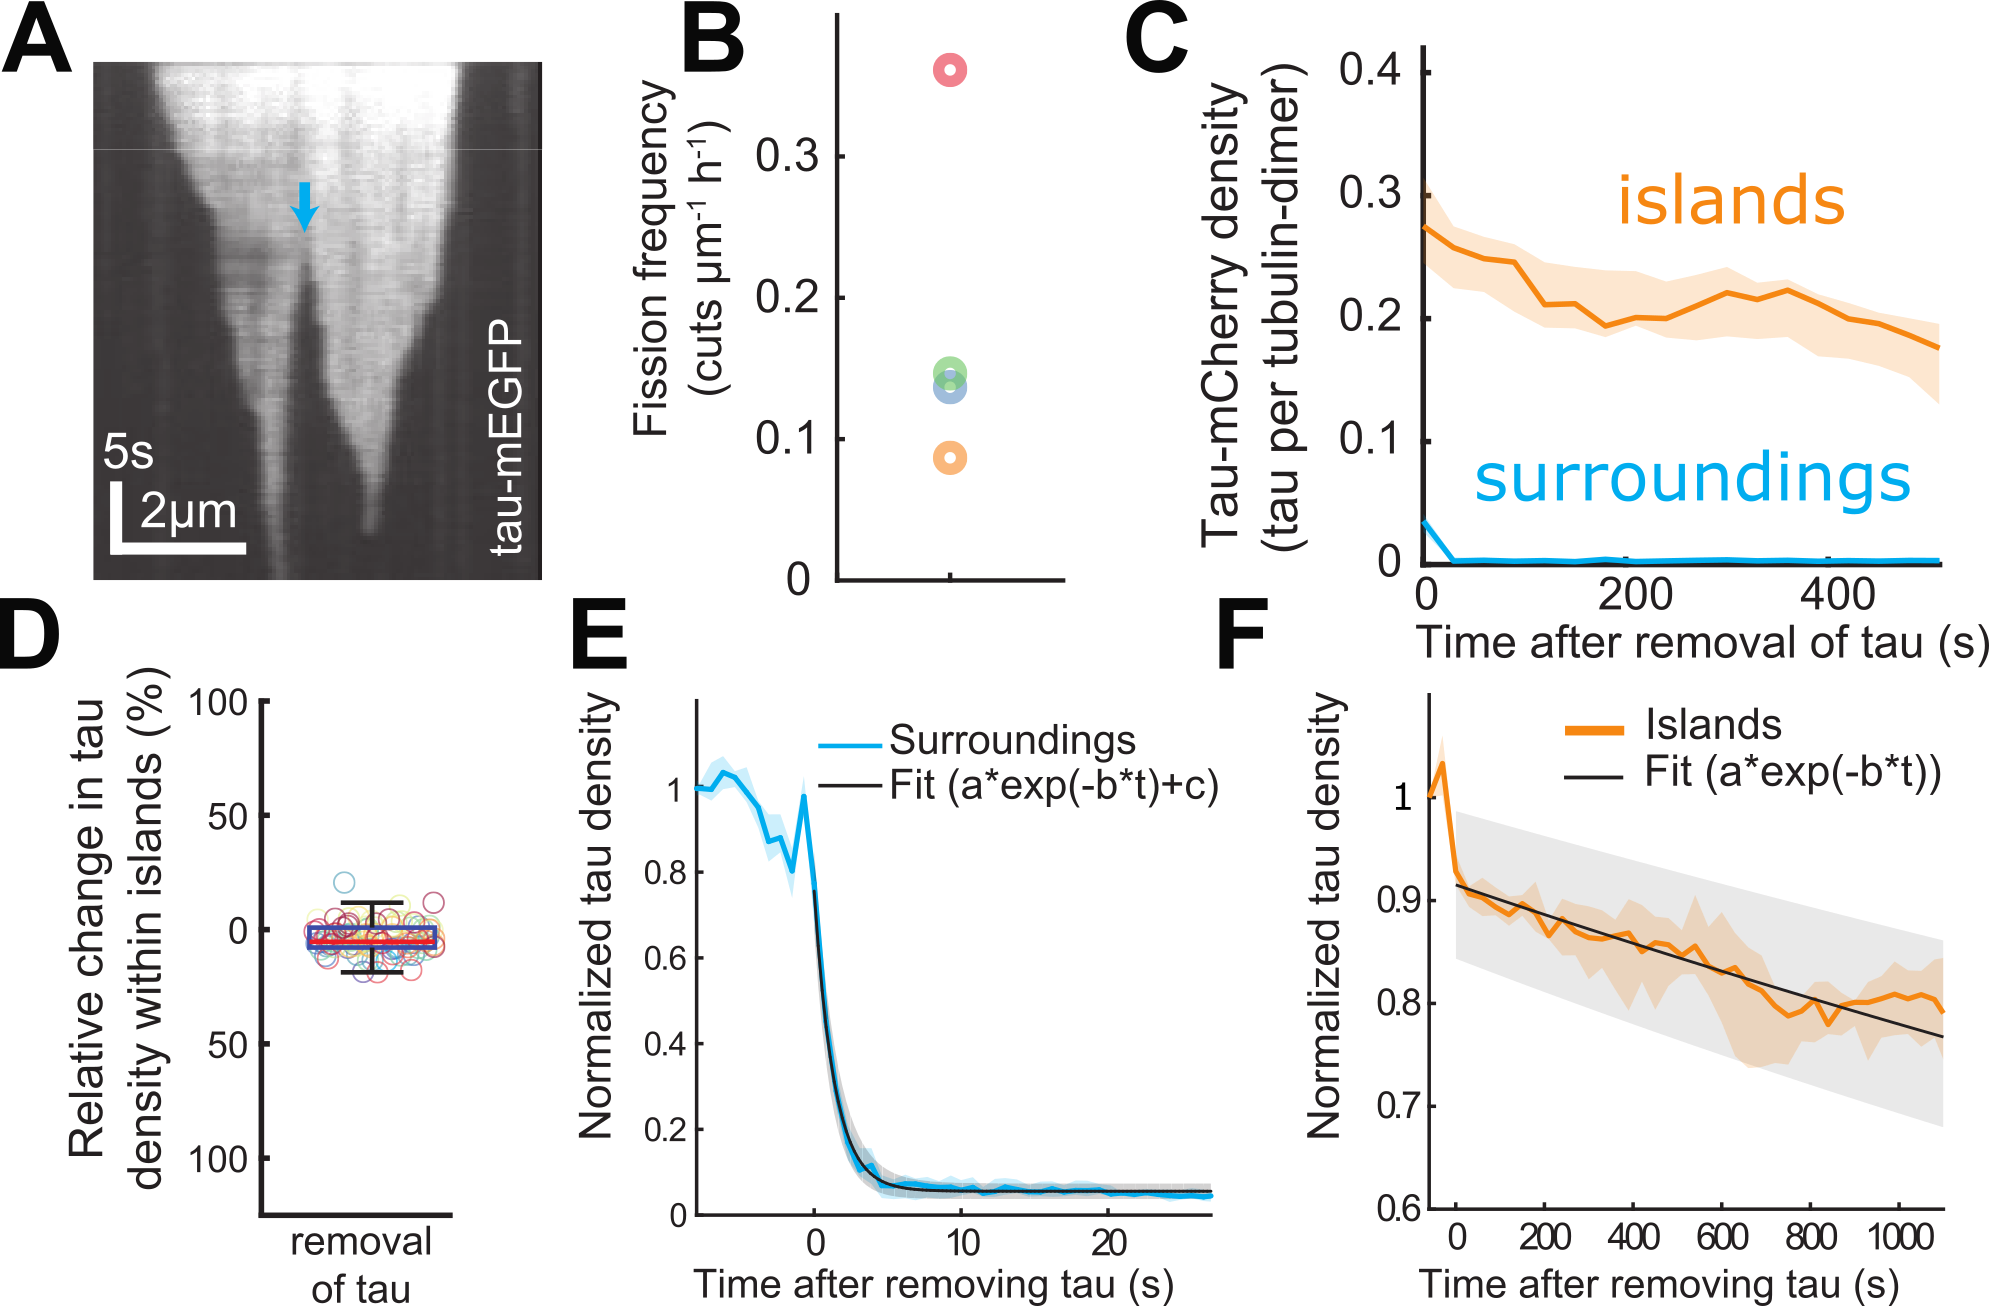
\includegraphics[width=1\linewidth]{Figures/tauSHRINK.png}
	\caption[Tau islands disassemble slowly upon the removal of tau from solution.]{
	\textbf{Tau islands disassemble slowly upon the removal of tau from solution.} (A) Kymograph showing the fluorescence signal of tau on the microtubule during the disassembly of the islands after the removal of tau from solution. The blue arrow indicates an exemplary fission event during island disassembly. (B) Frequency of fissions occurring within islands upon removal of tau from solution. Colors encode n = 4 experiments. (C) Distribution of island disassembly velocities upon removal of tau from solution. Colors encode experiments (same as in B), circles represent deassembly traces. (D) Exemplary time-trace of the tau density inside and outside the islands after the removal of (20nM) tau from solution (n = 9 microtubules). (E,F) Exemplary time-trace of tau density inside and tau density outside the islands after removal of (20nM) tau from solution, analogous to the results presented in E (n = 6 microtubules). Single exponential fits are indicated by solid lines. This experiment had been repeated 4 and 3 times for islands and surroundings, respectively, with similar results. In time-traces, thick lines and shaded areas indicate median and first and third quartiles, respectively. 
		}\label{tauSHRINK}
\end{wrapfigure}
Generally, the islands did not grow monotonously at their boundaries, but with variable velocities in the order of 25 nm/s, corresponding to about 10 molecules added per second \pref{tauGROW}{H}.  Importantly, the tau density in the islands stayed constant during the period of growth \pref{tauGROW}{I}, suggesting that the islands grow by the addition of tau molecules at their boundaries, reminiscent of epitaxial growth of thin films. As another indication that islands are formed by a well-defined tau layer occupying the entire accessible surface of the microtubule, we never observed an increase in the tau density when the boundaries of neighboring growing islands came into contact \pref{tauGROW}{C}.\par

When tau was removed from solution, the islands disassembled slowly from their boundaries, occassionally fissioning inside \pref{tauSHRINK}{A-B}. In contrast to island growth, this island shrinkage rarely halted \pref{tauSHRINK}{B}, and proceeded with a median velocity of approximately 2 tau molecules unbinding per second at a given island boundary \pref{tauSHRINK}{C}. Importantly, the tau density within islands only declined very slowly after removing tau from solution compared to the decline in tau density on all regions outside of islands (the “island surroundings”) \pref{tauSHRINK}{D}. Indeed, while in the surroundings tau unbound with a time constant of about 2 seconds as inferred from the decay of the fluorescence signal \pref{tauSHRINK}{E}, within the islands tau molecules unbound on the timescale of tens of minutes \pref{tauSHRINK}{F}. This extremely low unbinding rate explains the preservation of the islands in absence of tau in solution and suggests that the occasional island fissions observed during disassembly occur after rare events of tau molecules unbinding from inside the island. The large difference in the tau unbinding rates within islands compared to island surroundings, together with the assembly and disassembly kinetics at the island boundaries, indicate that tau molecules in the islands bind to microtubules cooperatively. 

\begin{figure}[b]
\centering
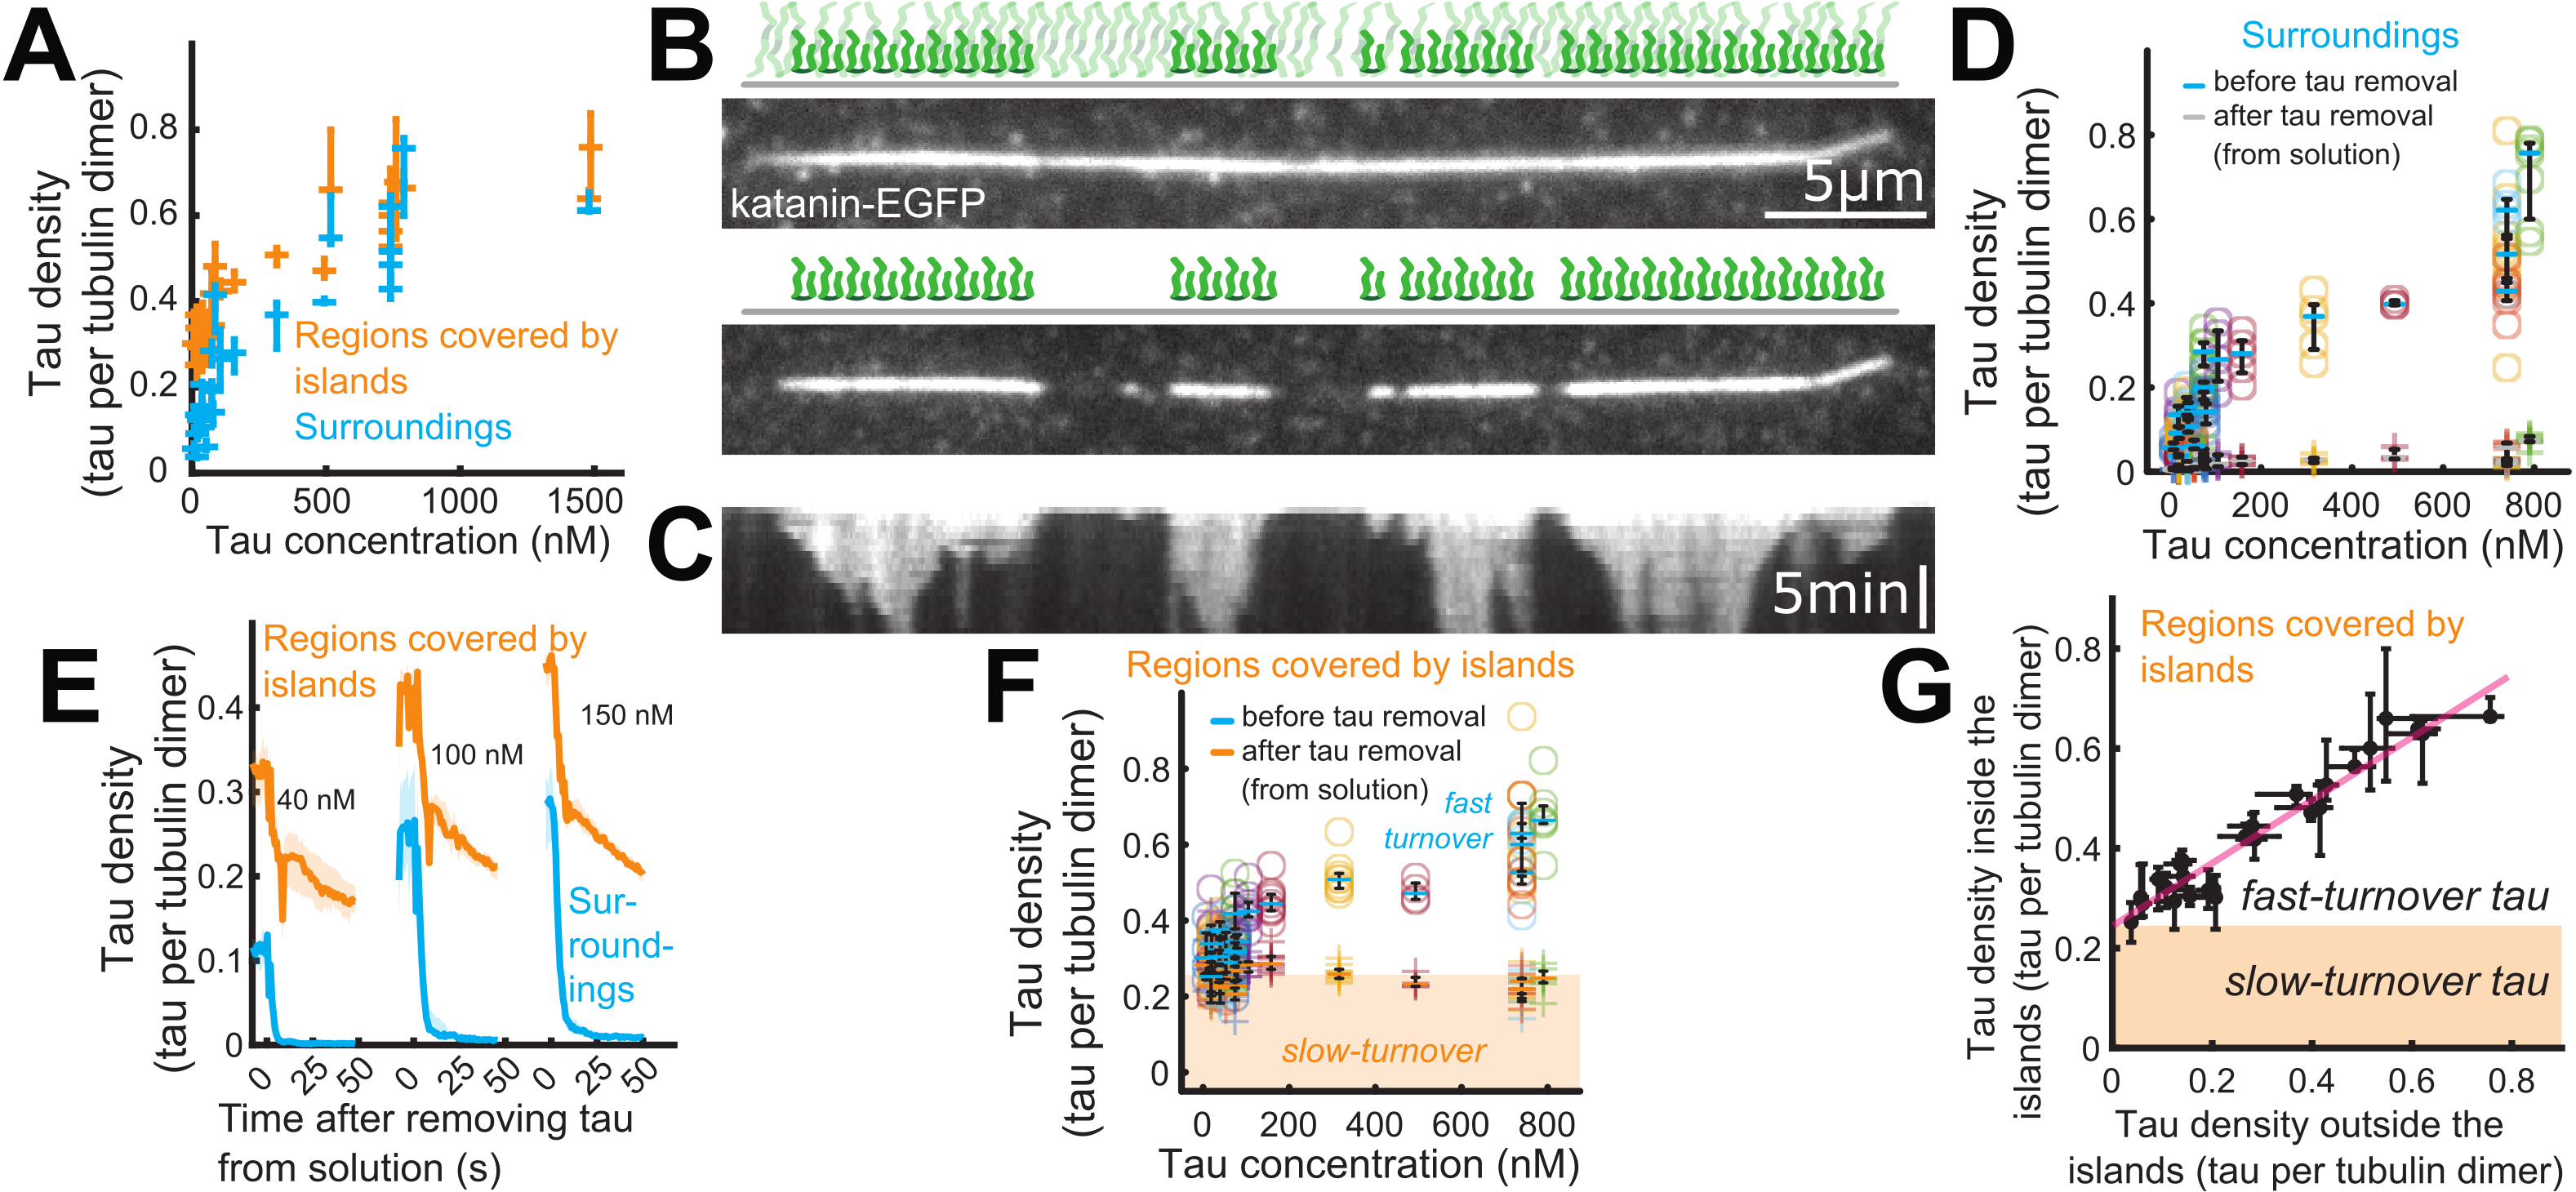
\includegraphics[width=1\linewidth]{Figures/tau_flushouts.png}
\caption[Tau islands are distinguished by tau cohesion.]{
\textbf{Tau islands are distinguished by tau cohesion.} (A) Fluorescence micrographs showing the coverage of a microtubule by tau. Upper panel: Uniform coverage at high (0.8 µM) concentration (5 minutes after the addition of tau). Lower panel: Islands (30 s after the removal of tau from solution). (B) The (equilibrium) density of tau on microtubules plotted against concentration of tau in solution. Horizontal lines indicate the three quartiles. (C) The (equilibrium) density of tau on microtubules inside island regions plotted against the density of tau in the surroundings, using the data presented in B. The red line visualizes a linear fit. (D) Kymograph of the experiment presented in A showing the disassembly of the islands after the removal of tau from solution. (E) Exemplary time-traces of tau density outside and inside the islands during subsequent cycles of i) addition of increasing concentrations of tau followed by ii) removal of tau from solution. Experiment such as presented in F and G. (F,G) Tau densities in regions covered by island and the surrounding regions established at various tau concentration, prior and after the removal of tau from solution. Points are color-coded by experiment, horizontal lines indicate the three quartiles of each experiment (in some panels the median is indicated by circle). In C and G, the characteristic island density (Main text, Methods) is indicated by the height of the shaded area.
	}\label{tauflushouts}
\end{figure}
To further explore the dynamics of tau molecules in the islands we formed islands using 20 nM tau-mCherry and, after 15 minutes, replaced the assay buffer by a solution containing 20 nM tau-mEGFP (Figure \ref{tau2}A). In the low-density regions, surrounding the islands, tau-mCherry rapidly dissociated from the microtubules with an average residence time of about 3 s (Figure \ref{tau_s2}D). This value is comparable to the residence time estimated for the situation discussed in Figure \ref{tau1}, where tau-mEGFP was completely removed from solution. By contrast, within the islands tau-mCherry dissociated markedly slower, with an average residence time of 30 seconds (Figures \ref{tau2}B, \ref{tau_s2}A). This value is, however, substantially faster than in the situation when tau was completely removed from solution (compare to Figure \ref{tau1}G and \ref{tau_s1}C). This observation demonstrates that tau unbinding from the islands depends on the tau concentration in solution (Figure \ref{tau2}C) and suggests that the underpinning interactions are multivalent, which, indeed, can be expected due to the presence of four microtubule binding repeats (4R) in the 2N4R tau molecules. Precedent for this observation are, for example, the concentration-dependent unbinding rates of multivalent DNA-binding proteins15. In the low-density regions surrounding the islands, tau-mEGFP molecules, in exchange for the leaving tau-mCherry, bound rapidly, while binding with a slower time constant into the islands (Figures \ref{tau2}A, \ref{tau2}B, \ref{tau_s2}A). Turnover from tau-mCherry to tau-mEGFP occurred uniformly and without any positional preferences along the whole lengths of both islands and their surroundings (albeit at different rates). Additionally, and similar to the initial formation of tau-mCherry islands, tau-mEGFP also associated with the boundaries of existing islands, elongating them (Figure \ref{tau2}A). To further study the spatio-temporal dynamics of tau in the high-density and low-density regions, we formed islands using a mixture of 20 nM tau-mCherry and 1 nM tau-mEGFP. This strategy allowed us to observe the motion of individual tau-mEGFP molecules in an environment dominated by tau-mCherry molecules. In the low-density regions, single tau-mEGFP molecules diffused rapidly (Figure \ref{tau2}E). By contrast, in the islands the tau-mEGFP molecules were bound stationarily to the microtubule surface (Figure \ref{tau2}E). Occasionally, single tau-mEGFP molecules initially diffusing outside an island became stationary when associating with an island boundary (Figure \ref{tau2}E). Combined, our results show that the tau molecules localizing in the islands are stationary, but can exchange with tau in solution.

\begin{figure}[h!]
\centering
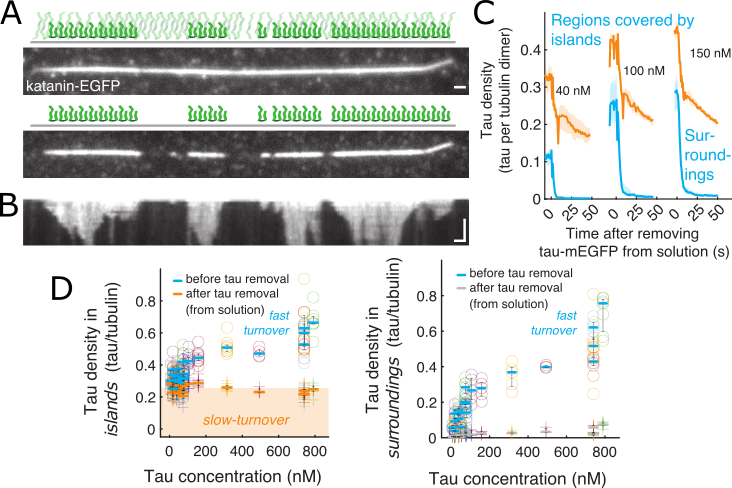
\includegraphics[width=1\linewidth]{Figures/tau5.png}
\caption[Tau molecules in the islands are stationary but exchange with tau in solution.]{
\textbf{Tau molecules in the islands are stationary but exchange with tau in solution.} 
	}\label{tau5}
\end{figure}
To explore the dependence of island formation on the concentration of tau we performed experiments with repeated cycles of i) microtubule incubation with increasing concentrations of tau-mEGFP followed by ii) tau-mEGFP removal from solution. Below a tau-mEGFP concentration of approximately 5 nM we did not observe any island formation (n = 245 microtubules in 5 experiments). Above this concentration, the tau-mEGFP density outside, as well as inside the islands, increased with increasing tau-mEGFP concentration in solution. After each removal of tau-mEGFP, the tau density in the regions surrounding the islands returned to the background level within several seconds (Figure \ref{tau5}C, consistent with the data shown in Figure \ref{tau1}H). By contrast, after each removal of tau-mEGFP, the tau density in the islands decayed in two stages: within a few seconds, a fast density drop occurred uniformly along the whole lengths of the islands, followed by a slow density decrease, the latter consistent with the data shown in Figure \ref{tau1}H (Figure \ref{tau5}C). Above a tau-mEGFP concentration of approximately 0.5 µM, the tau density on the microtubules reached saturation (Figure \ref{tau_s5}A) as reported before\parencite{Makrides2004}, suggesting that tau associates with a finite number of interaction sites on the microtubule. At this regime, the islands became apparent only after tau-mEGFP removal from solution, upon which tau-mEGFP rapidly unbound from the surroundings and islands became discernable (Figures \ref{tau5}A,B). Importantly, in all experiments, the tau-mEGFP density in the islands, after the fast density drop, had the same value of 0.26 ± 0.05 tau molecules per tubulin dimer (average ± SD, n = 101 microtubules, 14 experiments, Methods) independent of the initial tau concentration in solution (Figure \ref{tau5}D). Together with the results in Figures 1 and 2, these experiments show that cohesive islands on microtubules form by tau molecules that bind cooperatively and, in consequence, turn over slowly. At physiological tau concentrations\parencite{Wegmann} in the range of 0.5 - 1.5 µM, tau molecules, which turn over rapidly, co-localize with islands. These tau molecules, whose density depends on the tau concentration in solution in a similar way as the tau density outside the islands (Figure \ref{tau_s5}C), do not appear to participate in the cooperative island formation.

Because the N-terminus of tau mediates tau-tau interactions\parencite{Gamblin2003}, we repeated the described experiments with a truncated tau construct comprising the four-repeat microtubule-binding domain and the C-terminus but lacking the N-terminus (tau$\Delta$N-mEGFP, Figure TODO). Although tau$\Delta$N-mEGFP did interact with the microtubules, we did not observe any island formation even at tau$\Delta$N-mEGFP concentrations as high as 0.5 µM. To test the robustness of the island assembly using the full-length construct, we varied the ionic strength of the assay buffer and observed the islands to assemble over a broad range of conditions (0 - 125 mM KCl additional in the assay buffer). Combined, our results show that full-length human 2N4R tau on microtubules can separate into two kinetically distinct phases, namely islands of a high-density phase with very slow internal tau turn-over on the time scale of tens of minutes, surrounded by low-density regions with a fast tau turn-over on the time scale of seconds.

\subsection{Cooperatively bound tau uniquely interacts with microtubule motor proteins and cutting enzymes}
\begin{figure}[h!]
\centering
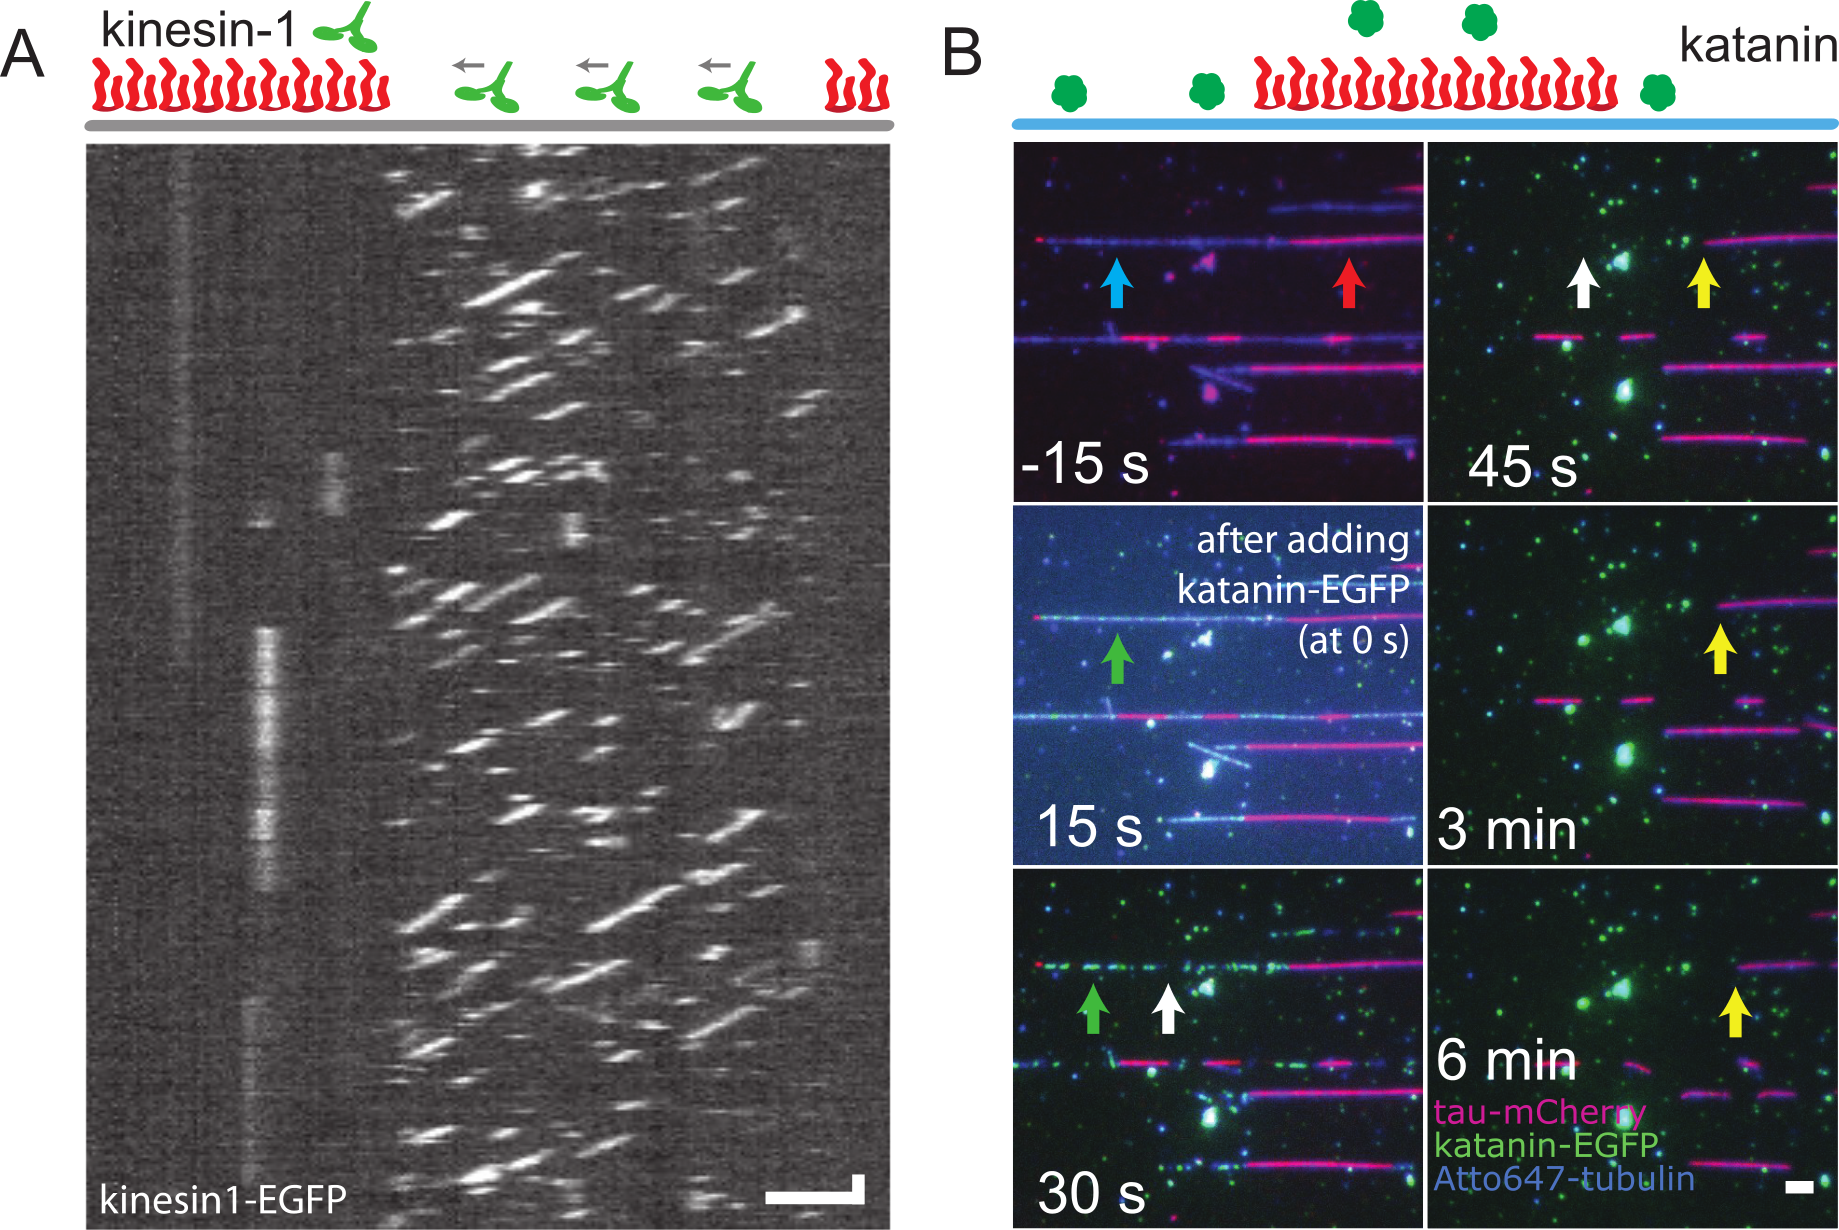
\includegraphics[width=1\linewidth]{Figures/tau3.png}
\caption[Tau islands constitute a protective sheath around microtubules.]{
\textbf{Tau islands constitute a protective sheath around microtubules.} (A) Intensity-inverted kymograph showing kinesin-1-GFP molecules bind to and move processively outside of the islands (the positions of the islands are indicated by schematics above the kymograph). We observed no kinesin-1-GFP binding within the island regions. When reaching the island boundaries, the kinesin-1-GFP molecules immediately dissociate from the microtubule. (B) Fluorescence micrographs showing the katanin-GFP-driven (green, position indicated by green arrow) severing of Atto-647-microtubules (blue) decorated with tau-mCherry islands (red, position indicated by red arrow) interspersed by regions of low tau-mEGFP density (indicated by blue arrow). Initially, microtubule severing and microtubule disassembly occurred only in the regions surrounding the islands (e.g. indicated by white arrow). On longer time scales (after approximately 1 minute), when the microtubule regions not protected by the islands already disassembled, katanin-GFP induced shortening of the island-covered regions of the microtubule (e.g. indicated by yellow arrow). Scale bars, vertical 2 s, horizontal 2 µm.   
	}\label{tau3}
\end{figure}
To investigate how the presence of tau islands affects the interaction of other proteins with microtubules, we formed tau islands using tau-mCherry and tested the interaction of other axonal MAPs with such tau-mCherry-decorated microtubules. First, we tested the processive microtubule-transport motor, kinesin-1. After addition of 60 nM kinesin-1 (GFP-tagged, dimerizing, truncated to be constitutively active, R. norvegicus kinesin-1: rKin-430-GFP) to microtubules in the presence of 20 nM tau-mCherry, we observed single motors moving processively through the low-density tau regions surrounding the islands. However, when reaching the boundary of a tau island, the motors dissociated instantaneously from the microtubule (Figure \ref{tau3}A). No motors bound to the tau islands from solution, resulting in rKin-430-GFP localizing solely to the surroundings of the islands. These results show that tau islands prevent kinesin-1-mediated transport along the microtubule surface. Second, we tested how the presence of islands affects the microtubule-severing enzyme katanin. After the addition of 100 nM katanin (GFP-tagged, M. musculus katanin p60/p80C: katanin-GFP\parencite{Jiang2017} to microtubules in the presence of 20 nM tau-mCherry, we observed katanin-GFP binding, severing and subsequent microtubule disassembly exclusively in the low-density tau regions surrounding the islands (Figure \ref{tau3}B). Only on longer time scales, the island-sheathed regions of the microtubules started to disassemble from their boundaries (Figure \ref{tau3}B), demonstrating that island-generated tau sheaths grant access to the microtubules only at their boundaries. Combined, these results show that tau islands constitute a protective sheath around the microtubule surface, which can hinder the activity of microtubule-severing factors and block kinesin-1-based transport. 

\begin{figure}[h!]
\centering
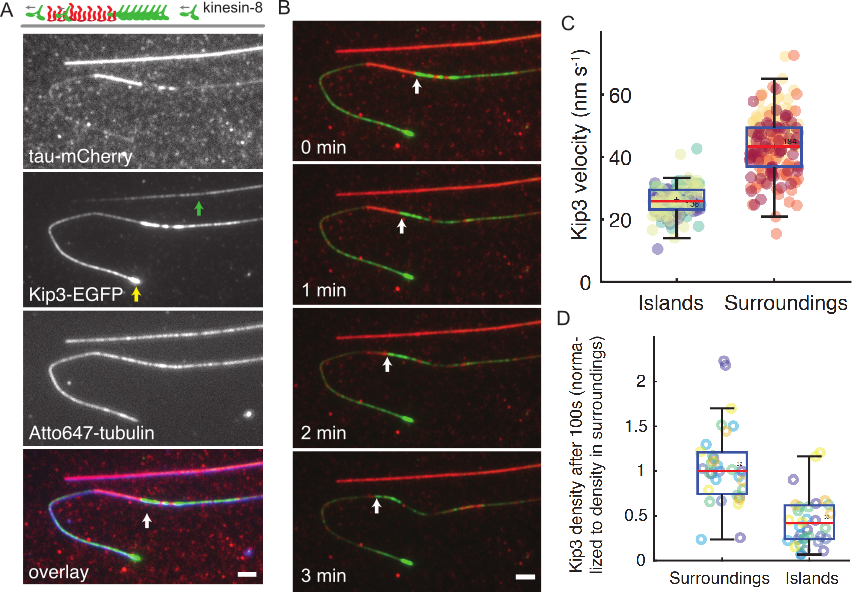
\includegraphics[scale=0.63]{Figures/tau4.png}
\caption[Tau islands can be regulated by super-processive kinesin motors.]{
\textbf{Tau islands can be regulated by super-processive kinesin motors.} (A) Multichannel fluorescence micrographs showing that kip3-GFP (kinesin-8, green) localizes in both regions, outside and within the tau-mCherry (red) islands (indicated by green arrow) on Atto-647-labeled microtubules (blue) and accumulates at the microtubule ends (yellow arrow) and in front of the islands (white arrow). (B) Multicolor timelapse micrographs showing that kip3-GFP (green) accumulating in front of the tau-mCherry island (red), can remove the island by displacing the tau-mCherry from the island edge (receding of the island boundary indicated by white arrow). (C) Quantification of velocities of single Kip3-GFP motors moving inside and outside the islands at 10 nM tau-mCherry in solution (n = 136 Kip3-GFP molecules inside islands, n = 184 outside, 3 experiments). (D) Quantification of Kip3-GFP density inside and outside the islands 100 s after the addition of Kip3-GFP (n = 98 microtubules in 6 experiments). The presented Kip3-GFP densities are normalized to the median of the density in the surroundings (within the same experiment).  Scale bars 2 µm.  
	}\label{tau4}
\end{figure}
To explore the effect of the tau islands on other kinesin family members, we turned to kinesin-8, which is involved in regulating axonal microtubule dynamics\parencite{KEVENAAR2016849}. S. cerevisiae Kip3, the best described member of the kinesin-8 family, pauses for extended periods of time when there is no available binding site within reach\parencite{Varga2009} resulting in its super-processivity\parencite{Varga2006} and the formation of traffic jams at the end of microtubules\parencite{Leduc2012}. Microtubule interaction sites of kinesin motor domains and the microtubule binding repeats of tau partially overlap\parencite{Kellogg2018}. We therefore wondered if (i) traffic jams would form in front of tau islands, where the Kip3 binding sites are occupied by the microtubule binding repeats of tau, and (ii) what effect high-density accumulations of molecular motors might have on tau islands. We thus tested the interaction of 45 nM Kip3-GFP with microtubules decorated with tau islands formed at 10 nM tau-mCherry. After the addition of Kip3-GFP, we observed that Kip3-GFP molecules could move in the low-density tau regions, like kinesin-1, and, in contrast to kinesin-1, also within the tau islands, albeit at a decreased velocity (Figure \ref{tau4}). Importantly, we observed that Kip3-GFP accumulated, in the direction of its movement, at the boundaries of the tau islands. Such high-density traffic jams of accumulated Kip3-GFP caused enhanced unbinding of tau-mCherry at these positions, eventually leading to the complete removal of the islands (Figures \ref{tau4}A,B and \ref{tau_s4}). The island displacement by Kip3 shows that not only do tau islands regulate the interaction of other MAPs with the microtubule surface but that, vice versa, the activity of other MAPs, such as super-processive motors proteins, can regulate the dynamics of the islands themselves.

\begin{figure}[h!]
\centering
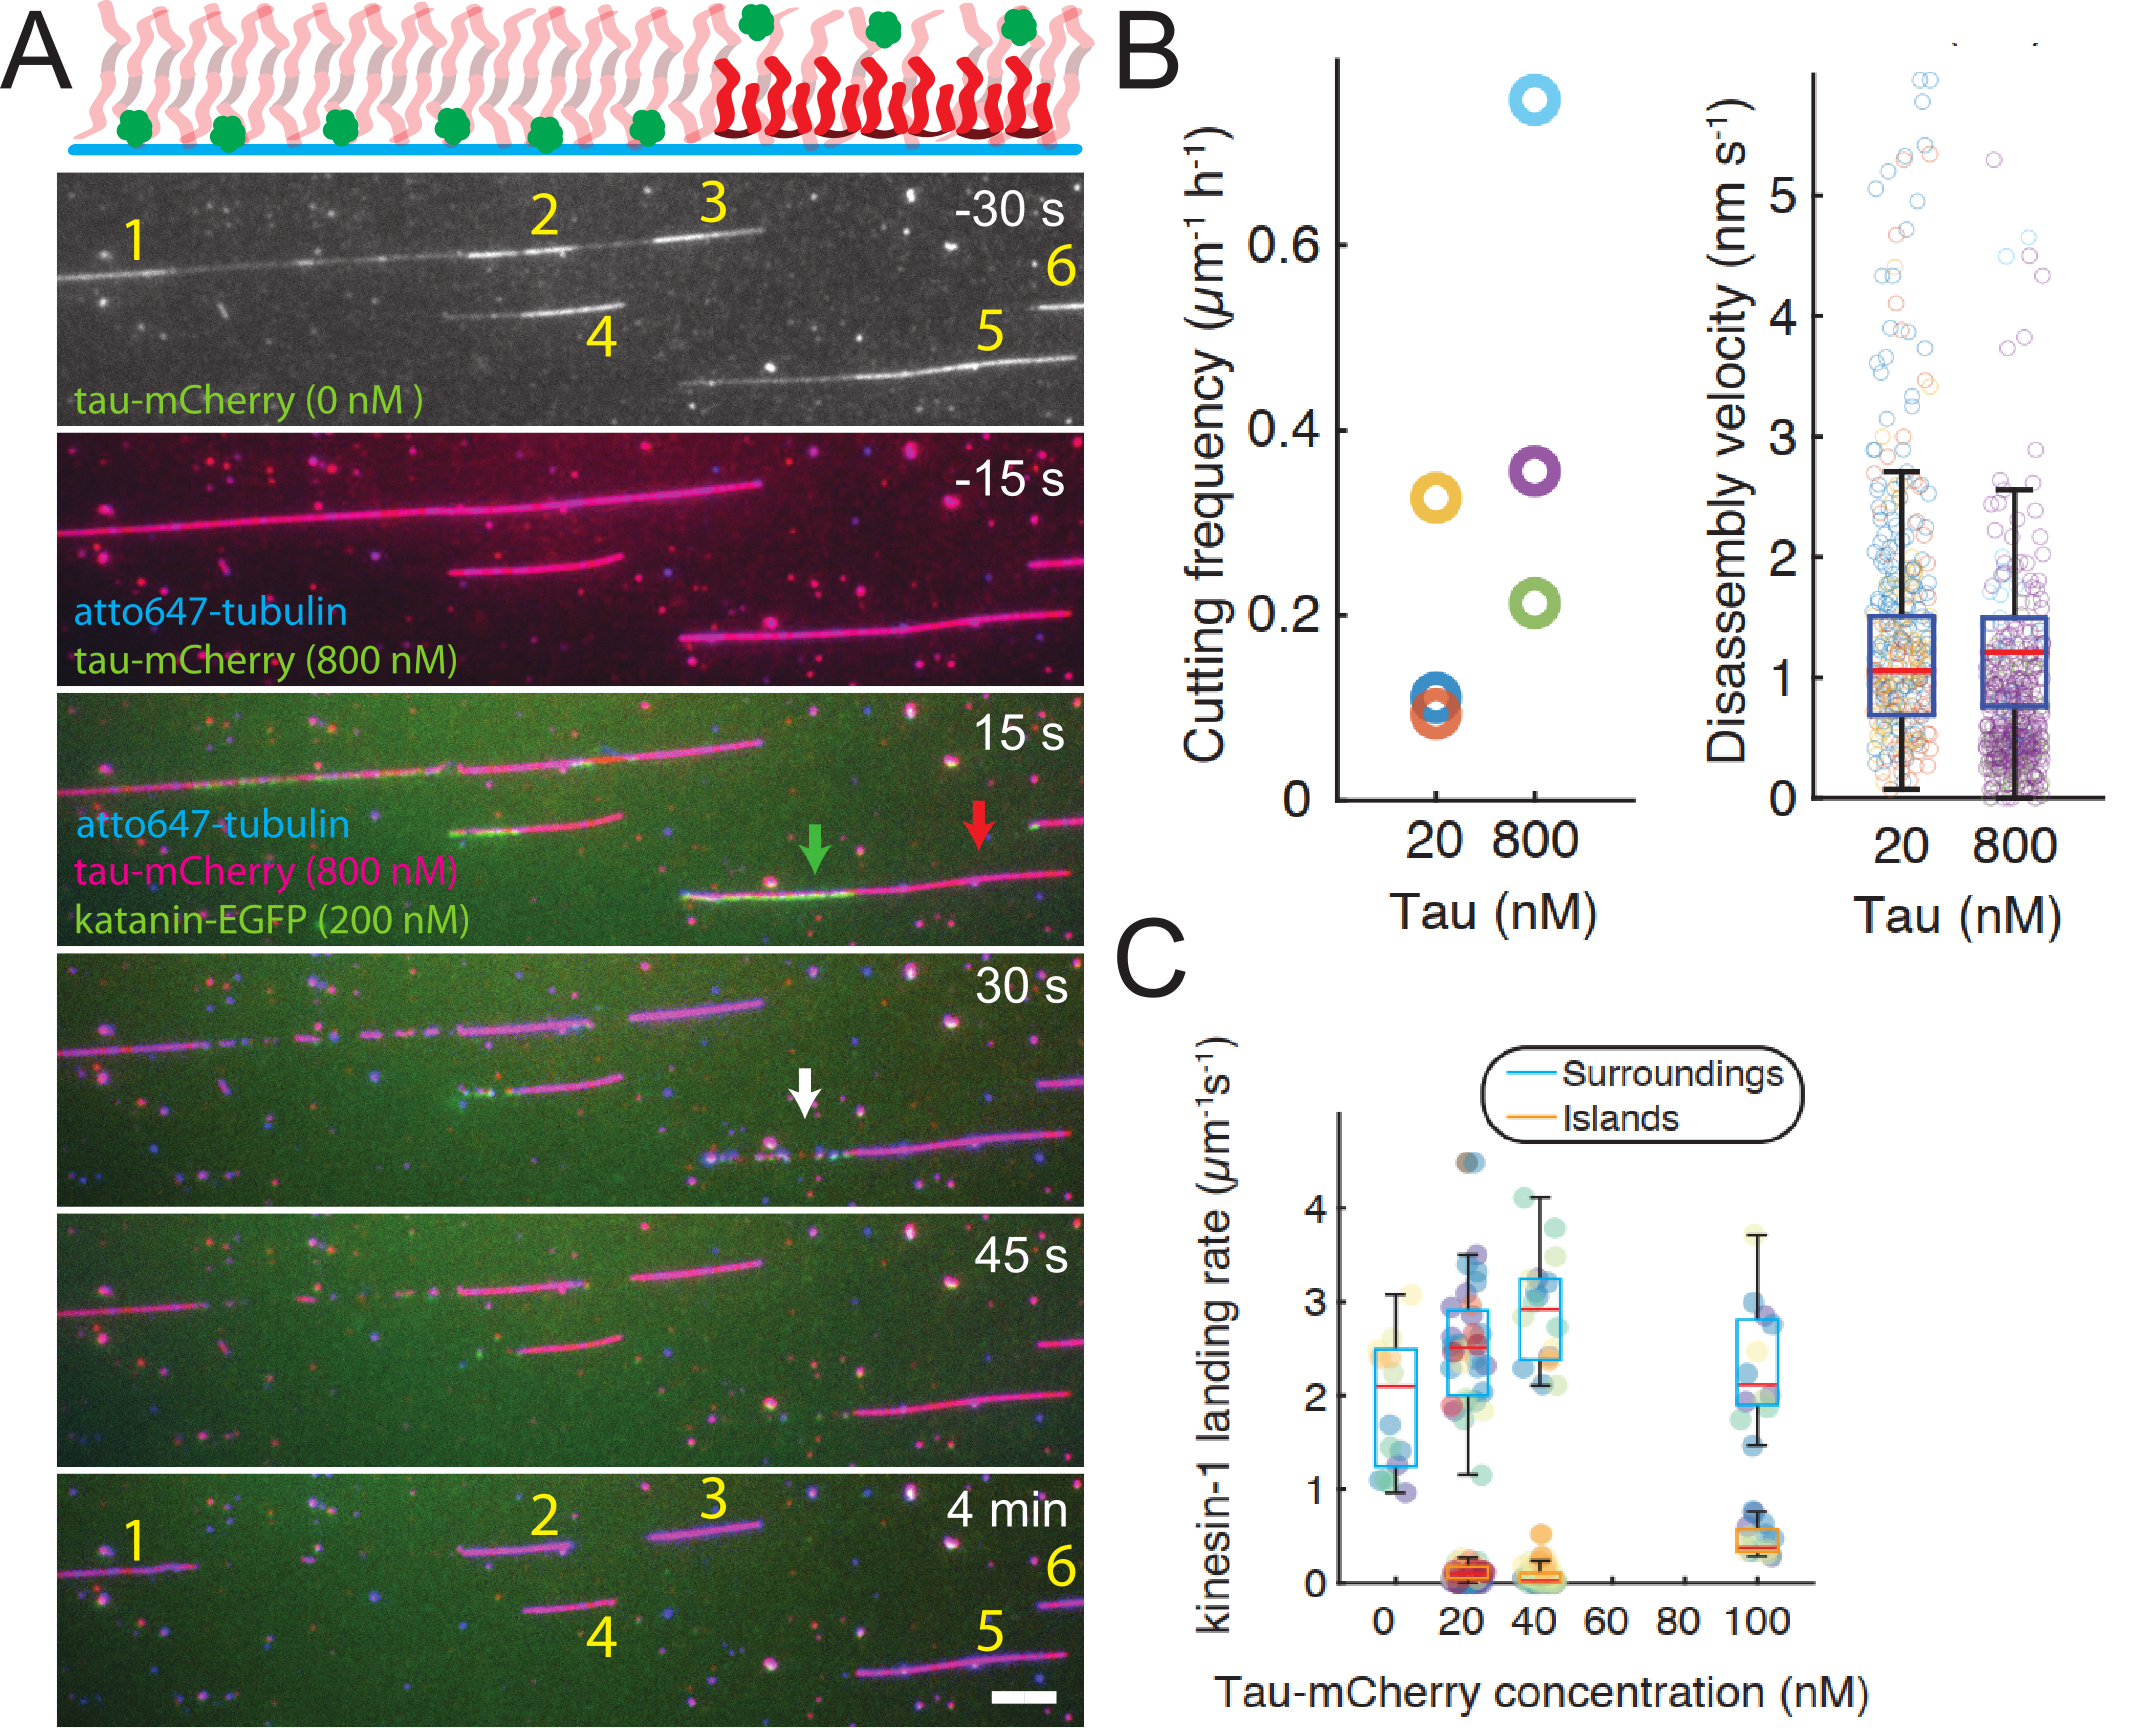
\includegraphics[width=1\linewidth]{Figures/tau6.png}
\caption[Microtubule shielding depends on tau cohesion of the islands.]{ 
\textbf{Microtubule shielding depends on tau cohesion of the islands.} (A) Fluorescence micrographs showing katanin-GFP-driven (green) severing of Atto-647-microtubules (blue) decorated with tau-mCherry islands (red) formed at 0.8 µM tau-mCherry concentration. The island positions (indicated by numbers) were determined by a brief removal of tau-mCherry from solution (Methods). Katanin is recruited to regions outside of the islands (green arrow) and excluded form the islands (red arrow). Microtubule severing and disassembly occurred initially only in the regions outside of the islands (example indicated by white arrow). Compare to the Figure \ref{tau3}B. Scale bar 2 µm. (B) Boxplot of katanin-mediated disassembly velocities of stretches of microtubules covered by tau islands (evaluated per island boundary) and the rate of katanin-generated cuts occurring within them. Experiments had been conducted at two different concentrations of tau in solution. (C) Kinesin-1 landing rates inside and outside the islands formed at various tau-mCherry concentrations in solution (7 experiments at 0 nM, 10 experiments at 20 nM, 7 experiments at 40 nM, 6 experiments at 100nM).
	}\label{tau6}
\end{figure}
 Since the characteristic tau density of the islands is lower than that of the surrounding regions at physiological tau concentrations (Figure 5), we wondered if the discretely binding tau molecules in the island surroundings, at these concentrations, are sufficient for shielding the microtubule against microtubule severing. To test the shielding against katanin severing at physiological tau concentration we thus formed tau-mCherry islands at saturating conditions (0.8 µM). After 5 minutes of incubation we briefly removed tau-mCherry from solution to note the position of the islands, and then again re-introduced 0.8 µM tau-mCherry in the assay. We then exposed such tau-mCherry decorated microtubules to 0.2 µM katanin-GFP analogously to the experiment presented in Figure \ref{tau3}B. Strikingly, we observed qualitatively identical results as in the Figure \ref{tau3}B. Namely, regions surrounding the islands and occupied by the diffusible tau-mCherry phase were severed and rapidly disassembled, while microtubule regions shielded by the islands persisted (Figure \ref{tau6}). This shows that the density of tau on the microtubule surface is not the factor determining the shielding function of tau. Rather it is the cohesion between the tau molecules constituting the islands, which protects the microtubules. This conclusion is supported by our observation that increasing the tau concentration in solution did not substantially increase shielding against tau (Figure \ref{tau6}B) and kinesin-1 (Figure \ref{tau6}B). 

\subsection{Tau islands do not form at regions of high microtubule curvature}
\begin{figure}[h!]
\centering
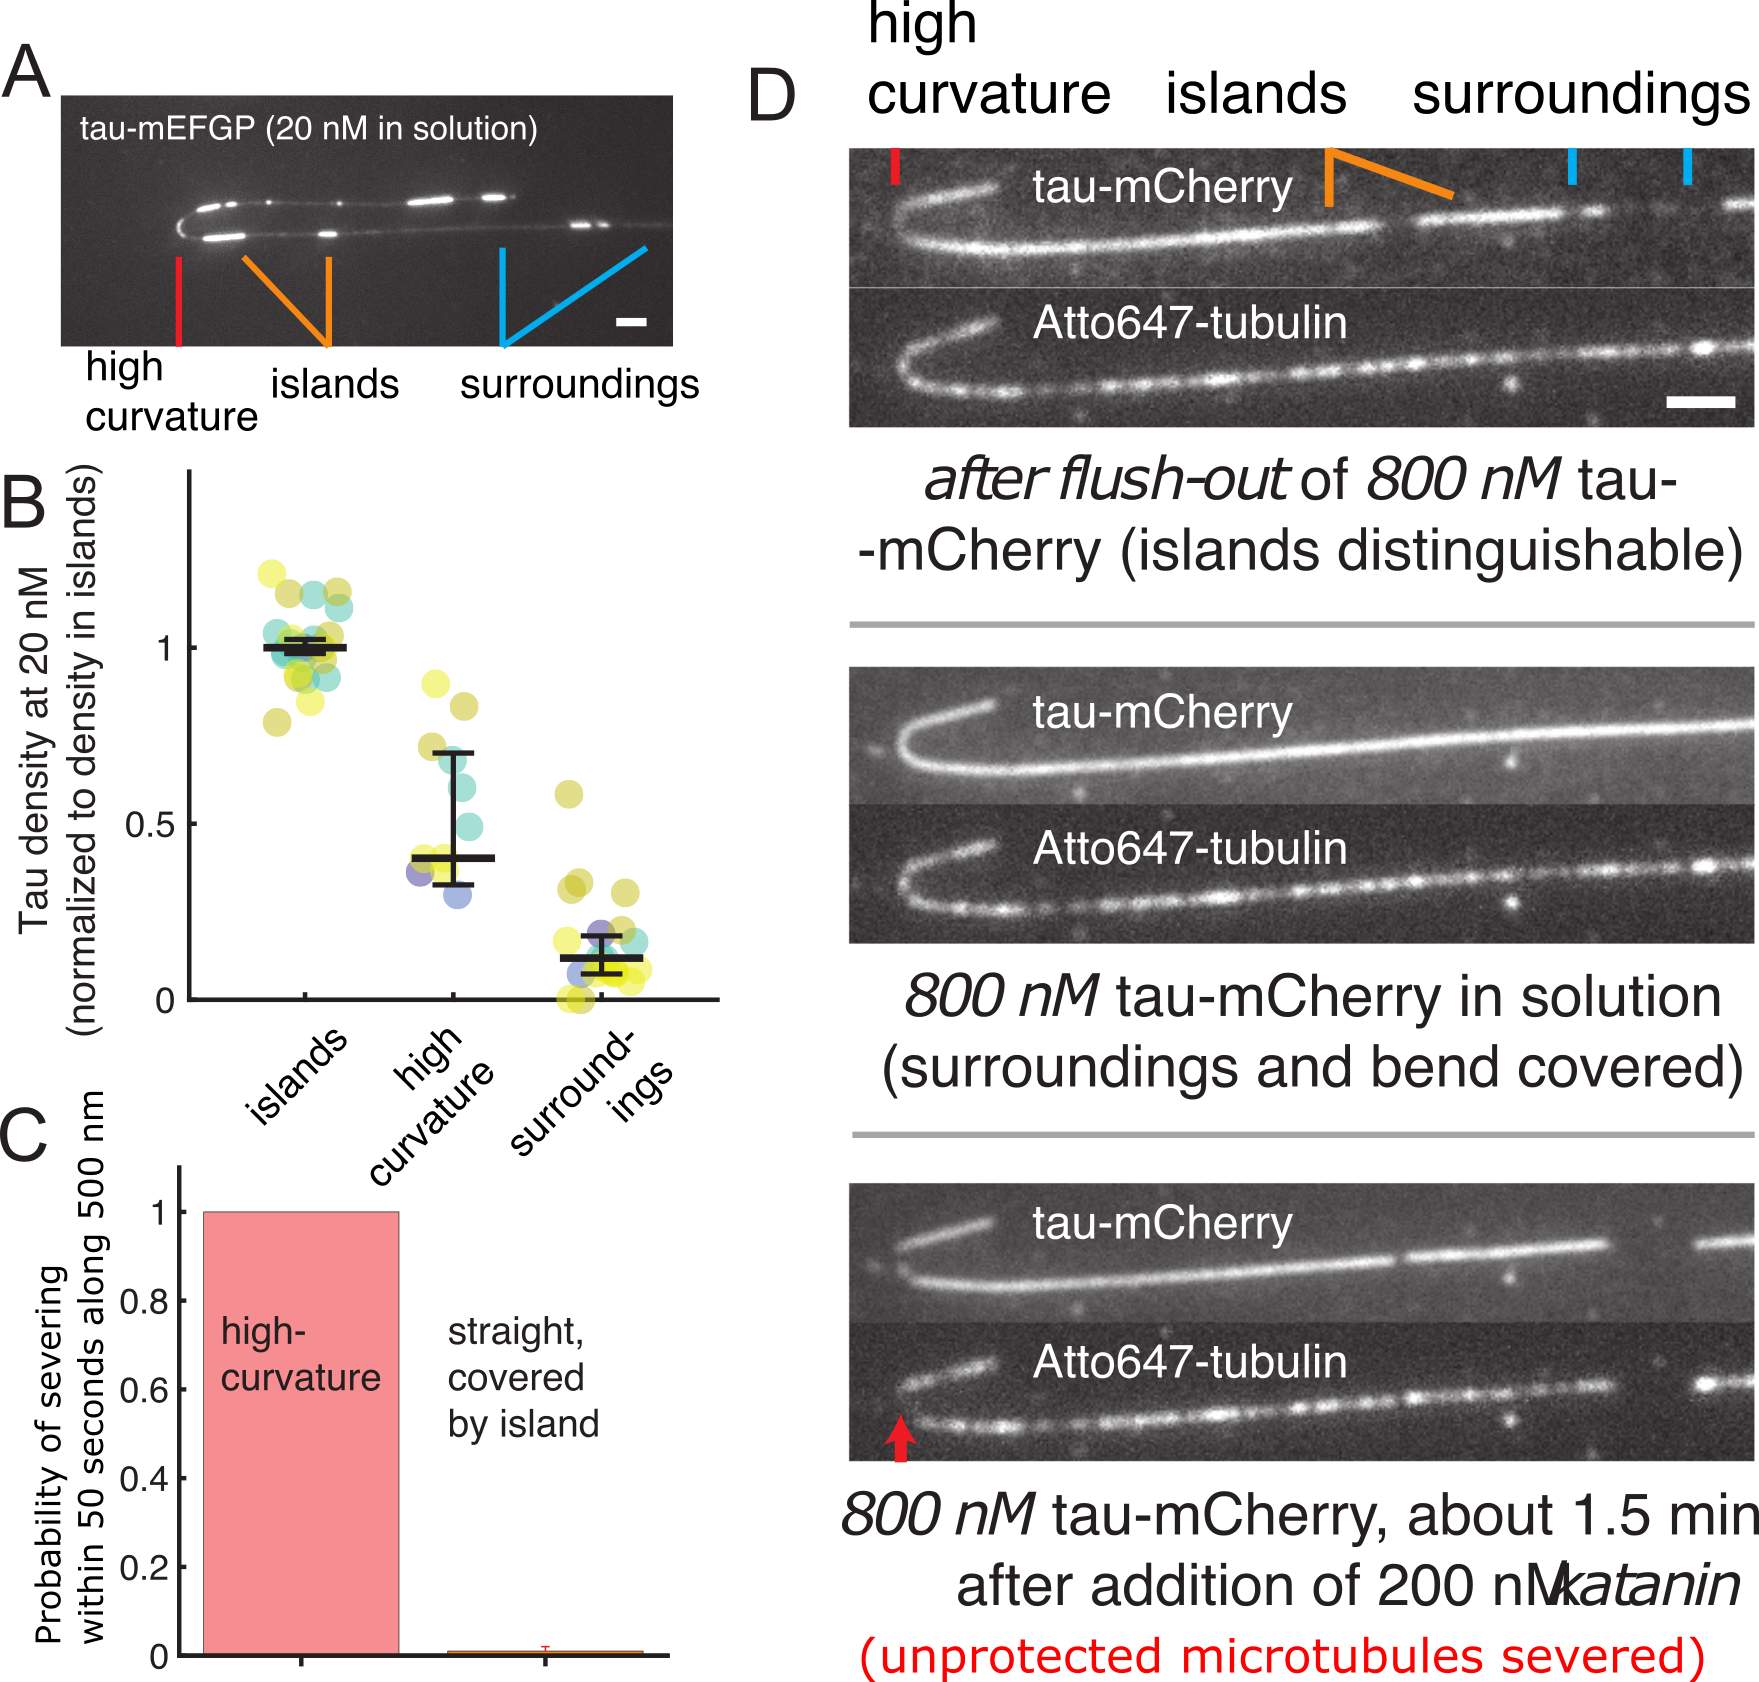
\includegraphics[scale=1]{Figures/tau7.png}
\caption[Tau islands do not form at regions of high microtubule curvature.]{
\textbf{Tau islands do not form at regions of high microtubule curvature.} (A) Fluorescence micrograph showing the tau-mEGFP signal on microtubules at 20 nM tau-mEGFP in solution. Tau islands have higher tau-mEGFP densities than the tau-mEGFP regions localizing to microtubule regions with high curvature. (B) Densities of tau-mEGFP outside the islands, inside the islands and in the regions of high curvature at 20 nM tau-mEGFP in solution (n = 11 high-curvature regions in 5 experiments). Points are color-coded by experiments, horizontal lines indicate the three quartiles, weighted such that each experiment has equal weight. (C) Probability of severing of highly curved microtubule regions and adjacent straight island-covered microtubule regions, within 150 s after the addition of katanin. The bars represent the probability averaged over n = 4 experiments (29 bends and 82 straight microtubules), error bars represent the S.D. Curved microtubule regions were always cut. (D) An experiment as analyzed in (C). Tau-mCherry islands on microtubules after the removal of 800 nM tau-mCherry from solution (upper panel); the same microtubule in presence of re-introduced 800 nM tau-mCherry in solution (middle panel); the same microtubule in presence of 200 nM katanin-GFP and 800 nM tau-mCherry. The red arrow highlights that the high curvature region  had been cut by katanin. This experiment had been repeated 4 times with similar results. Scale bars 2 µm.
	}\label{tau7}
\end{figure}
Earlier reports show that tau preferentially localized to highly-curved microtubules\parencite{Samsonov2004}. We indeed observed that regions of highly curved microtubules (radius < 2.5 µm) exhibited a tau density that was higher than in the surroundings, but lower than in the islands on straight microtubule regions (Figure \ref{tau7}A,B). The tau bound to highly curved microtubule regions also did not unbind as quickly as in the surroundings (Figure \ref{tau7}D, \ref{tau_s7}A,B). Importantly however, the highly curved regions were not protected from katanin-mediated severing (Figure \ref{tau7}C,D), demonstrating that tau molecules in the highly curved regions do not form a cohesive layer. Accordingly, in the curved regions tau-mEGFP binding was distinct from the island formation on straight microtubules, in that there was no growth at boundaries (Figure \ref{tau_s7}C). Combined, these experiments suggest that high curvatures of microtubules, though attracting tau, prevent the formation of cohesive tau islands.